Para descomponer un número en factores primos solo basta con seguir la idea aprendida en enseñanzas anteriores ejemplo:

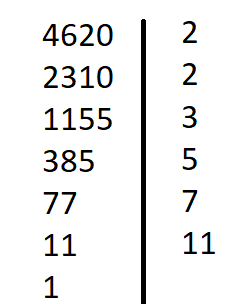
\includegraphics[scale=0.4]{img/descomposicion_primos}

En esta caso $4620=2^{2}*3^{1}*5^{1}*7^{1}*11^{1}$


\subsection{Probando división}
Este es el algoritmo más básico para encontrar una factorización prima.

Dividimos por cada divisor posible $d$. Se puede observar que es imposible que todos los factores primos de un número compuesto $n$ ser más grande que $\sqrt{n}$. Por lo tanto, sólo necesitamos probar los divisores $2 \le d \le \sqrt{n}$.

El divisor más pequeño debe ser un número primo. Eliminamos el número factorizado y continuamos el proceso. Si no podemos encontrar ningún divisor en el rango $[2; \sqrt{n}]$, entonces el número en sí tiene que ser primo.

\subsubsection{Factorización de rueda}
Esta es una optimización de la división de prueba. Una vez que sabemos que el número no es divisible por 2, no necesitamos verificar otros números pares. Esto nos deja sólo $50\%$ de los números a comprobar. Después de factorizar 2 y obtener un número impar, podemos simplemente comenzar con 3 y contar solo los demás números impares.

Este método se puede ampliar aún más. Si el número no es divisible por 3, también podemos ignorar 
todos los demás múltiplos de 3 en cálculos futuros. Entonces solo necesitamos verificar los 
números $5,~7,~11,~13,~17,~19,~23,~\dots$. Podemos observar un patrón de estos números restantes. 
Necesitamos verificar todos los números con $d \bmod 6 = 1$ y $d \bmod 6 = 5$. Entonces esto nos 
deja sólo con $33,3\%$ por ciento de los números a verificar. Podemos implementar esto 
factorizando primero los números primos 2 y 3, después de lo cual comenzamos con 5 y solo 
contamos los restos $1$ y $5$ módulo $6$.

Si continuamos ampliando este método para incluir aún más números primos, se pueden alcanzar mejores porcentajes, pero las listas de omisión serán más grandes.

\subsubsection{Primos precalculados}

Extendiendo el método de factorización de la rueda indefinidamente, solo nos quedarán números primos para verificar. Una buena forma de comprobarlo es precalcular todos los números primos con el criba de Eratóstenes hasta que $\sqrt{n}$ y pruébelos individualmente.

\subsubsection{Factorización de N}

Una buena manera de verificar es precalcular todos los números primos con la criba de Eratóstenes hasta $\sqrt{N}$ y probarlos individualmente.

Para un factor primo $p$ de $N$, la multiplicidad de $p$ es el máximo exponente $a$ para el cual $p^a$ es un divisor de $N$. La factorización de un número entero es una lista de los factores primos de ese número, junto con su multiplicidad. El Teorema fundamental de la Aritmética establece que todo número entero positivo tiene una factorización de primos única.

\subsubsection{Factorización de N!}

Que pasa si ahora queremos descomponer N! la idea básica seria iterar desde 1 hasta N e ir descomponiendo cada número acumulando las potencias o hallar N! y luego descomponerlo, pero esto tendría una complejidad de O($N* \sqrt{N}$) el cual sería muy costoso para valores muy grandes de N. Analicemos la siguiente idea:

10!=1*2*3*4*5*6*7*8*9*10 Necesitamos hallar cuantos 2 hay.

\begin{tabular}{|c|c|c|c|c|c|c|c|c|c|c|c|}
	\hline 
	10!& 1 & 2 & 3 & 4 & 5 & 6 & 7 & 8 & 9 & 10 & total \\ 
	\hline 
	Descomposición de n1& 1 & 2 & 3 & 2$^{2}$ & 5 & 2*3 & 7 & 2$^{3}$ & 3$^{2}$ & 2*5 &  \\ 
	\hline 
	Primo 2& 0 & 1 & 0 & 2 & 0 & 1 & 0 & 3 & 0 & 1 & 8 \\ 
	\hline 
	Primo 3& 0 & 0 & 1 & 0 & 0 & 1 & 0 & 0 & 2 & 0 & 4 \\ 
	\hline 
\end{tabular} 

\hspace{0.5em}

Para el caso del 2 seria todos los múltiplos de 2 hasta N ejemplo para 10 hay 5 que seria 10/2 luego todos los múltiplos de 4 hasta N que sería N/4 y así hasta que la potencia de 2 sea mayor que N la suma de estos seria el exponente de la potencia de 2 luego de descomponer N!, en  este caso sería 2$^{10/2+10/4+10/8}$=2$^{5+2+1}$=2$^{8}$ y este sería el procedimiento para todos los primos hasta N.



\subsection{Método de factorización de Fermat}
Podemos escribir un número compuesto impar $n = p \cdot q$ como la diferencia de dos cuadrados $n = a^2 - b^2$:

$$n = \left(\frac{p + q}{2}\right)^2 - \left(\frac{p - q}{2}\right)^2$$

El método de factorización de Fermat intenta explotar este hecho adivinando el primer cuadrado 
$a^2$, y comprobando si la parte restante, $b^2 = a^2 - n$, también es un número cuadrado. Si es 
así, entonces hemos encontrado los factores $a-b$ y $a+b$ de $n$.

\subsection{Método de Pollard $P-1$}
Es muy probable que al menos un factor de un número sea $B$-powersmooth para $B$ pequeños. $B$-powersmooth significa que cada potencia primaria $d^k$ que divide $p-1$ es es como máximo $B$. Por ejemplo, la factorización prima de $4817191$ es $1303 \cdot 3697$ . Y los factores son $31$-powersmooth y $16$-powersmooth respetablemente, porque  $1303 - 1 = 2 \cdot 3 \cdot 7 \cdot 31$ y $3697 - 1 = 2^4 \cdot 3 \cdot 7 \cdot 11$. En 1974, John Pollard inventó un método para extraer $B$-powersmooth factores  de un número compuesto.

La idea surge del pequeño teorema de Fermat . Sea una factorización de $n$  ser $n = p \cdot q$ . Dice que si $a$ es coprimo a $p$ , se cumple la siguiente afirmación:

$$a^{p - 1} \equiv 1 \pmod{p}$$

Esto también significa que

$$a^{(p - 1)^k} \equiv a^{k \cdot (p - 1)} \equiv 1 \pmod{p}.$$

Entonces para cualquier $M$ con $p - 1 ~|~ M$ sabemos que $a^M \equiv 1$. Esto significa que  $a^M - 1 = p \cdot r$, y por eso también $p ~|~ \gcd(a^M - 1, n)$.

Por lo tanto, si $p-1$ por un factor $p$ de $n$ divide $M$, podemos extraer un factor usando el algoritmo de Euclides.

Está claro que el más pequeño $M$ que es múltiplo de cada $B$-powersmooth numero es $\text{lcm}(1,~2~,3~,4~,~\dots,~B)$. O alternativamente:

 $$M = \prod_{\text{prime } q \le B} q^{\lfloor \log_q B \rfloor}$$
 
Aviso, si $p-1$ divide $M$ para todos los factores primos $p$ de $n$ , entonces $\gcd(a^M - 1, n)$ solo será $n$. En este caso no recibimos ningún factor. Por lo tanto, intentaremos realizar el $\gcd$ varias veces, mientras calculamos $M$.

Algunos números compuestos no tienen $B$-powersmooth factores para pequeños B . Por ejemplo, los factores del número compuesto $100~000~000~000~000~493 = 763~013 \cdot 131~059~365~961$ son $190~753$-powersmooth y $1~092~161~383$-powersmooth. Tendremos que elegir $B >= 190~753$ para factorizar el número

Observe que este es un algoritmo probabilístico. Una consecuencia de esto es que existe la posibilidad de que el algoritmo no pueda encontrar
ningún factor.

\subsubsection{Algoritmo $\rho$ de Pollard}

El algoritmo Rho de Pollard es otro algoritmo de factorización de John Pollard.  Sea la factorización prima de un número $n = p q$. El algoritmo analiza una secuencia pseudoaleatoria. $\{x_i\} = \{x_0,~f(x_0),~f(f(x_0)),~\dots\}$ dónde $f$ es una función polinómica, generalmente $f(x) = (x^2 + c) \bmod n$  es elegido con $c = 1$.

En este caso no nos interesa la secuencia $\{x_i\}$ . Estamos más interesados en la secuencia. $\{x_i \bmod p\}$. Desde $f$ es una función polinómica y todos los valores están en el rango $[0;~p)$, esta secuencia eventualmente convergerá en un bucle. La paradoja del cumpleaños en realidad sugiere que el número esperado de elementos es $O(\sqrt{p})$ hasta que comience la repetición. Si $p$ es más pequeña que $\sqrt{n}$, la repetición probablemente comenzará en $O(\sqrt[4]{n})$.


Aquí hay una visualización de tal secuencia $\{x_i \bmod p\}$ con $n = 2206637$, $p = 317$, $x_0 = 2$ y $f(x) = x^2 + 1$. Por la forma de la secuencia se puedever muy claramente por qué el algoritmo se llama algoritmo $\rho$ de Pollard.

% TODO: \usepackage{graphicx} required
\begin{figure}[h!]
	\centering
	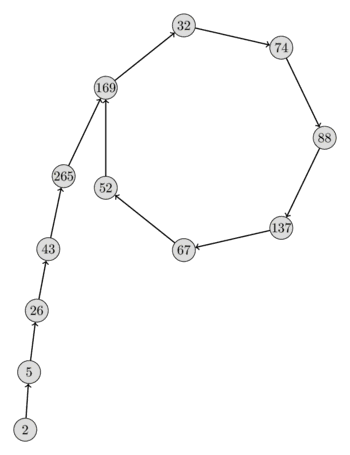
\includegraphics[width=0.35\linewidth]{img/pollard_rho}
	
	\label{fig:pollardrho}
\end{figure}


Sin embargo, todavía queda una pregunta abierta. ¿Cómo podemos explotar las propiedades de la secuencia? $\{x_i \bmod p\}$ a nuestra ventaja sin siquiera saber el número $p$ ¿sí mismo?

En realidad es bastante fácil. Hay un ciclo en la secuencia $\{x_i \bmod p\}_{i \le j}$ si y sólo si hay dos índices $s, t \le j$ tal que $x_s \equiv x_t \bmod p$. Esta ecuación se
puede reescribir como $x_s - x_t \equiv 0 \bmod p$ que es lo mismo que $p ~|~ \gcd(x_s - x_t, n)$.

Por tanto, si encontramos dos índices $s$  y $t$ con $g = \gcd(x_s - x_t, n) > 1$ , hemos encontrado un ciclo y también un factor  $g$ de $n$. Es posible que $g = n$.
En este caso no hemos encontrado un factor adecuado, por lo que debemos repetir el algoritmo con un parámetro diferente (valor inicial diferente $x_0$ , constante diferente $c$ en la función polinómica $f$ ).

Para encontrar el ciclo, podemos utilizar cualquier algoritmo de detección de ciclo común.

\subsubsection{Algoritmo de búsqueda de ciclos de Floyd}
Este algoritmo encuentra un ciclo utilizando dos punteros que se mueven sobre la secuencia a 
diferentes velocidades. Durante cada iteración, el primer puntero avanzará un elemento, mientras 
que el segundo puntero avanzará a todos los demás elementos. Usando esta idea es fácil observar que 
si hay un ciclo, en algún momento el segundo puntero se encontrará con el primero durante los 
bucles. Si la duración del ciclo es $\lambda$ y el $\mu$ es el primer índice en el que comienza el 
ciclo, entonces el algoritmo se ejecutará en O$(\lambda + \mu)$ tiempo.

Este algoritmo también se conoce como algoritmo de la liebre y la tortuga , basado en el cuento en el que una tortuga (el puntero lento) y una liebre (el puntero más rápido) tienen una carrera.

De hecho, es posible determinar el parámetro $\lambda$ y $\mu$ usando este algoritmo (también en 
O($\lambda + \mu$) tiempo y O$(1)$ espacio). Cuando se detecta un ciclo, el algoritmo devolverá 
verdadero . Si la secuencia no tiene un ciclo, entonces la función se repetirá sin cesar. Sin 
embargo, esto se puede evitar utilizando el algoritmo Rho de Pollard.

La siguiente tabla muestra los valores de $x$ y $y$ durante el algoritmo para $n = 2206637$ , $x_0 = 2$ y $c = 1$.

$$
\newcommand\T{\Rule{0pt}{1em}{.3em}}
\begin{array}{|l|l|l|l|l|l|}
	\hline
	i & x_i \bmod n & x_{2i} \bmod n & x_i \bmod 317 & x_{2i} \bmod 317 & \gcd(x_i - x_{2i}, n) \\
	\hline
	0   & 2       & 2       & 2       & 2       & -   \\
	1   & 5       & 26      & 5       & 26      & 1   \\
	2   & 26      & 458330  & 26      & 265     & 1   \\
	3   & 677     & 1671573 & 43      & 32      & 1   \\
	4   & 458330  & 641379  & 265     & 88      & 1   \\
	5   & 1166412 & 351937  & 169     & 67      & 1   \\
	6   & 1671573 & 1264682 & 32      & 169     & 1   \\
	7   & 2193080 & 2088470 & 74      & 74      & 317 \\
	\hline
\end{array}
$$

Como se dijo anteriormente, si $n$ es compuesto y el algoritmo devuelve $n$ como factor, hay que repetir el procedimiento con diferentes parámetros $x_0$ y $c$. Por ejemplo, la elección $x_0 = c = 1$ no factorizará $25 = 5 \cdot 5$. El algoritmo volverá $25$. Sin embargo, la elección $x_0 = 1$, $c = 2$ lo factorizará.


\subsubsection{Algoritmo de Brent}

Brent implementa un método similar al de Floyd, utilizando dos punteros. La diferencia es que en lugar de avanzar los punteros uno y dos lugares respectivamente, avanzan potencias de dos. Tan pronto como $2^i$ es mayor que $\lambda$ y $\mu$ , encontraremos el ciclo.


La combinación de una división de prueba para números primos pequeños junto con la versión de Brent del algoritmo rho de Pollard crea un algoritmo de factorización muy potente.

